\documentclass[12pt]{book}
\usepackage[utf8]{inputenc}
\usepackage[T1]{fontenc}
\usepackage[spanish]{babel}
\setlength{\parindent}{0cm}
\usepackage[a4paper,top=3cm,bottom=2cm,left=3cm,right=3cm,marginparwidth=1.75cm]{geometry}
\usepackage{graphicx}
\usepackage{float}
\usepackage{alltt}
\title{Implementación de un Sistema de Monitoreo de Equipos de Red con Nagios }
\author{Emanuel David Cortes Antonio}
\setlength{\parskip}{10pt}
\begin{document}
  \maketitle
  \tableofcontents
  
  \chapter{Desarrollo}

  \section{Instalación y Configuración del sistema operativo con Nagios Core  }
  \subsection{Instalación del Sistema operativo} 
    La instalación y configuración de Nagios Core puede variar según la elección del sistema operativo, para esta implementación se optó
    por CentOS que es un sistema Linux basado en RedHat y las principales características de su elección son que es software libre y que
    esta distribución está orientada a los servicios de Red.
    \begin{figure}[htb]
      \centering
        
\includegraphics[width=0.8\textwidth]{./Imagenes/centos-7-logo}
      \caption{CentOS v7} \label{fig:CentOS}
    \end{figure}

    Después de descargar e instalar CentOS en el servidor es necesario configurar la interfaz de red para tener salida a internet y poder
    actualizar algunos repositorios y así tener una correcta instalación de Nagios Core.
    \vspace{-5mm}
    \begin{alltt} 
      \input{./txt/interfacered.txt}
    \end{alltt}
  \subsection{Ajustes previos del sistema operativo }
    Se necesitan realizar algunos ajustes al sistema operativo que permitirán la instalación de paquetes y ejecución correcta de Nagios.
    \begin{alltt}
      \input{./txt/ajustesso.txt}
    \end{alltt} 
    \subsection{Instalación de dependencias para compilar Nagios }
    Es necesario preparar el sistema operativo con los paquetes de software que Nagios Core requiere para ser instalado, se deben introducir
    los siguientes comandos como usuarios root en la terminal para ser instalados:
    \begin{alltt}
      \input{./txt/centospackage.txt}
    \end{alltt} 
    \subsection{Instalación de Nagios y plugins }
    Lo primero que hay que hacer es descargar los archivos de instalación, para ello navegamos al sitio oficial y descargamos los paquetes de
    Nagios Core y Nagios plugins en su última versión:
      \begin{alltt}
        \input{./txt/descarga.txt}
      \end{alltt} 
      Ya con los archivos tar.gz descargados, es necesario dirigirse a la ruta donde se encuentran y será necesario descomprimirlo y compilarlo
      para ello se ingresarán los siguientes comandos en la terminal:
    \begin{alltt}
      \input{./txt/nagiosinst.txt}
    \end{alltt}
    \begin{figure}[htb]
      \centering
        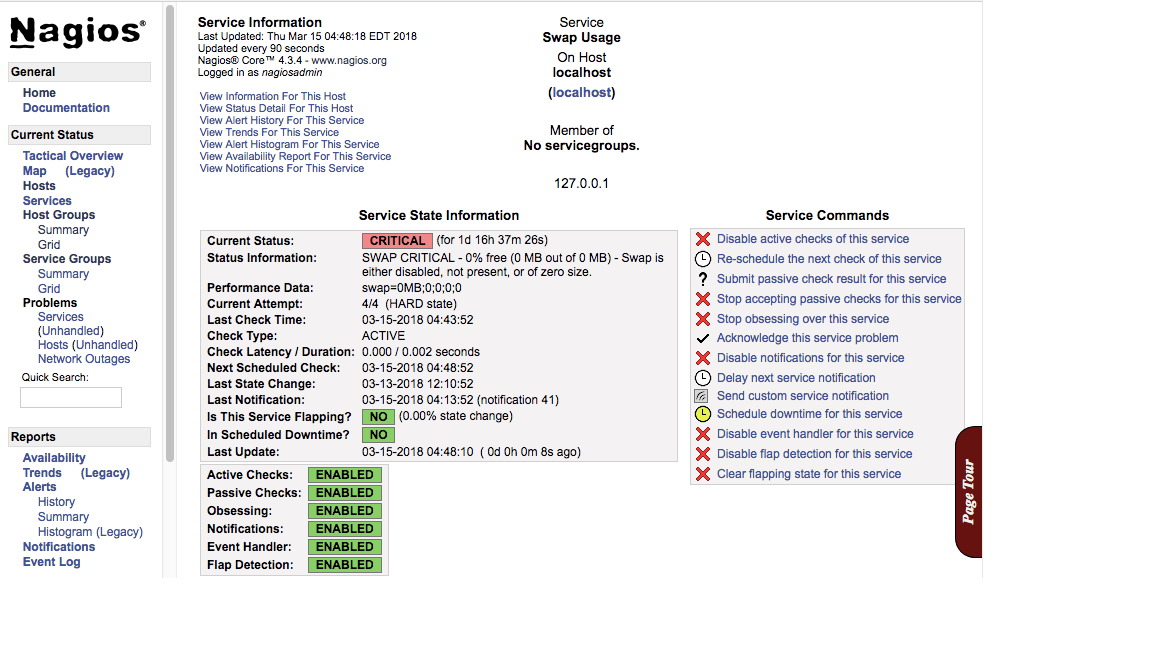
\includegraphics[width=0.8\textwidth]{./Imagenes/nagios.png}
      \caption{Nagios Core Página de inicio} \label{fig:NagiosCorte}
    \end{figure}
      Nagios es un sistema de monitorización con multiples servicios y por ello a la hora de configurar alguno en especifico podria haber un error
      el cual seria muy complejo detectar, para solucionar este problema y especificar algun servicio que se desee agregar (un servidor, switvh o router)
      se dispone de un paquete oficial de plugins en la pagina de Nagios Core:
    \begin{alltt}
      \input{./txt/plugins.txt}
    \end{alltt} 
    \section{Agregar Equipos a Nagios}
    \subsection{ Definición de objecto en Nagios}
    Los switches y routers pueden ser monitorizados por Nagios, la forma mas sencilla para determinar perdidas de paquetes es "pingueandolos" y con agentes
    SNMP el inconveniente con esta última forma es que no todos los equipos de red lo soportan, por ello para esta implementación se optó por utilizar sólo 
    pings.

    En Nagios a las definiciones de hosts, contactos, servicios, comandos y otros se le conoce como objetos.
    La definición de objetos en Nagios se realiza a través de archivos con extensión ".cfg", la definición de estos archivos puede ser en cualquier parte de 
    los directorios pero por convención y recomendación se pueden ubicar en la ruta {\itshape /usr/local/nagios/etc/objects } estos archivos ademas deben ser
    incluidos en la dirección {\itshape /usr/local/nagios/etc/nagios.cfg } en el cual estan las rutas de todos los objetos agregados.
    Sin embargo, Nagios ya trae unos cuantos archivos agregados en la ruta {\itshape /usr/local/nagios/etc/objects } para la definicion de los objectos, estos
    serviran como especies de plantillas para distintos servicios como servidores windows, linux, switches y routers.
    \subsection{ Definiendo un Host }
    Lo primero será definir el host:
    \begin{alltt}
      \input{./txt/definehost.txt}
    \end{alltt}
    \begin{enumerate}
      \item {\bf use: } Con esta directiva se le indica una plantilla de la que heredar la configuración. En caso de
      conflicto porque una misma directiva se utilice tanto en la plantilla como en la definición del host,
      siempre tendrá prioridad el valor que se establece en la definición host. De momento usaremos esta
      plantilla y más adelante las veremos más detalladamente. 
      \item {\bf host\_name: }Nombre corto usado para identificar al host.
      \item {\bf alias: } Nombre o descripción usada para identificar al host.
  
      \item {\bf address: } Dirección IP del equipo a monitorizar.
  
      \item {\bf hostgroups: } Nombre del hostgroup al que pertenece. 
      \item {\bf icon\_image: } Agregar un icono al equipo en la página principal.
      \item {\bf statusmap\_image: } Agregar un icono en el indice del host.
    \end{enumerate}
    Aquí se pueden establecer muchas más directivas, y no todos los hosts tienen que estar definidos de la
    misma forma. Unos pueden tener unos valores y unas directivas, y otros otras. Incluso se puede evitar la
    utilización de plantillas, aunque siempre se deben incluir algunas directivas que son obligatorias, ya sean
    puestas explícitamente o heredadas de una plantilla. 
    \subsection{ Definiendo un HostGroup }
    En Nagios la definición de la directiva hostgroup no es obligatoria pero puede ser util a la hora de visualizar
    los equipos en la interfaz web ya que se pueden agrupar o facilitar la getión en algun servicio que será aplicado
    a todos los hosts de un determinado hostgroup.
    \vspace{-5mm}
    \begin{alltt}
      \input{./txt/definegroup.txt}
    \end{alltt}
    \vspace{-5mm}
    Un hostgruop solo necesita dos directivas, el nombre y el alias.
    \subsection{ Definiendo los servicios }
    Son muchos los servicios que Nagios incluye para monitorear como se menciono anteriormente como algun servidor con
    sistema operativo windows o Linux, o en este caso un equipo de red.
    \vspace{-15mm}
    \begin{alltt}
      \input{./txt/defineservice.txt}
    \end{alltt}
    \vspace{-10mm}
    \begin{enumerate}
      \item {\bf use: } Como en el caso de la definición del host, esta directiva se emplea para utilizar una plantilla,
      en este caso “generic-service”.

      \item {\bf host\_name: } Es el nombre del host o hosts a los que se le aplicará la monitorización de este
      servicio. Si quisiéramos especificar un hostgroup podríamos hacerlo utilizando la directiva
      hostgroup\_name en su lugar. Si lo hiciéramos ya no sería obligatorio el uso de la directiva
      host\_name.
      \item {\bf service\_description: } Nombre descriptivo para el servicio.
      \item {\bf check\_command: } El comando que usará este servicio junto con su variable, en este caso “check\_ping”.
      \item {\bf check\_interval: } Es el intervalo de tiempo que se espera para recibir una respuesta del comando, por default 
      una unidad son 60 segundos.
      \item {\bf retry\_interval: } Es el intervalo de tiempo que se espera para reintentar ejecutar el comando en caso 
                                    que la respuesta del comando sea negativa.

    \end{enumerate}

    \section{ Modificando la Interfaz Web }
    Ahora que ya tenemos instalado y agregados equipos a Nagios Core nos queda configurar la interfaz web en la que se podrán observar
    la monitorización de los servicios para ello es necesario acceder a la ruta {\itshape /usr/local/nagios/share } que es donde se 
    encuentra la plantilla por defecto y es aqui donde se sustituye o se modifican los archivos html y css.
    \begin{figure}[H]
      \centering
        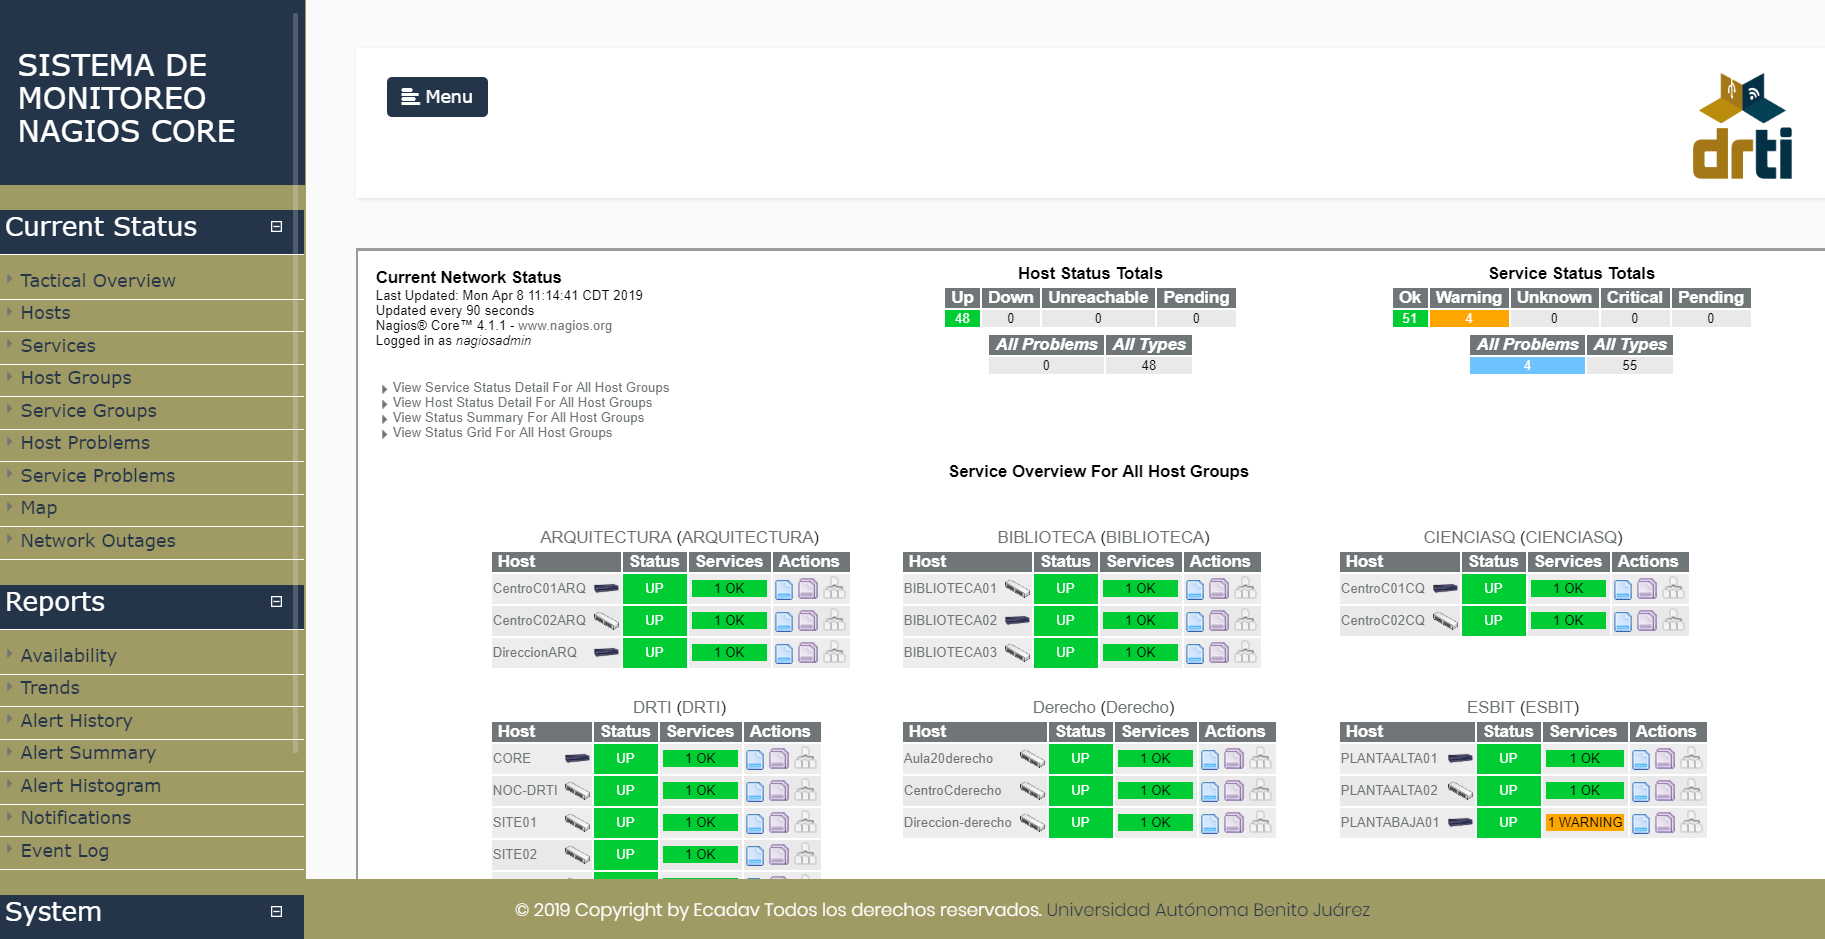
\includegraphics[width=0.8\textwidth]{./Imagenes/interfaz.png}
      \caption{Nueva interfaz web de Nagios} \label{fig:Nagios-DRTI}
    \end{figure}

    Se opto por un diseño básico sin muchas modificaciones a la interfaz inicial, pero que incluyera una pequeña descripción del lugar
    en donde se implemento el sistema de monitoreo, ademas que el diseño fuera responsivo para poderse adaptar a todo tipo de tamaño de
    pantallas en los diferentes dispositivos con los que se cuentan.
    \begin{figure}[htb]
      \centering
        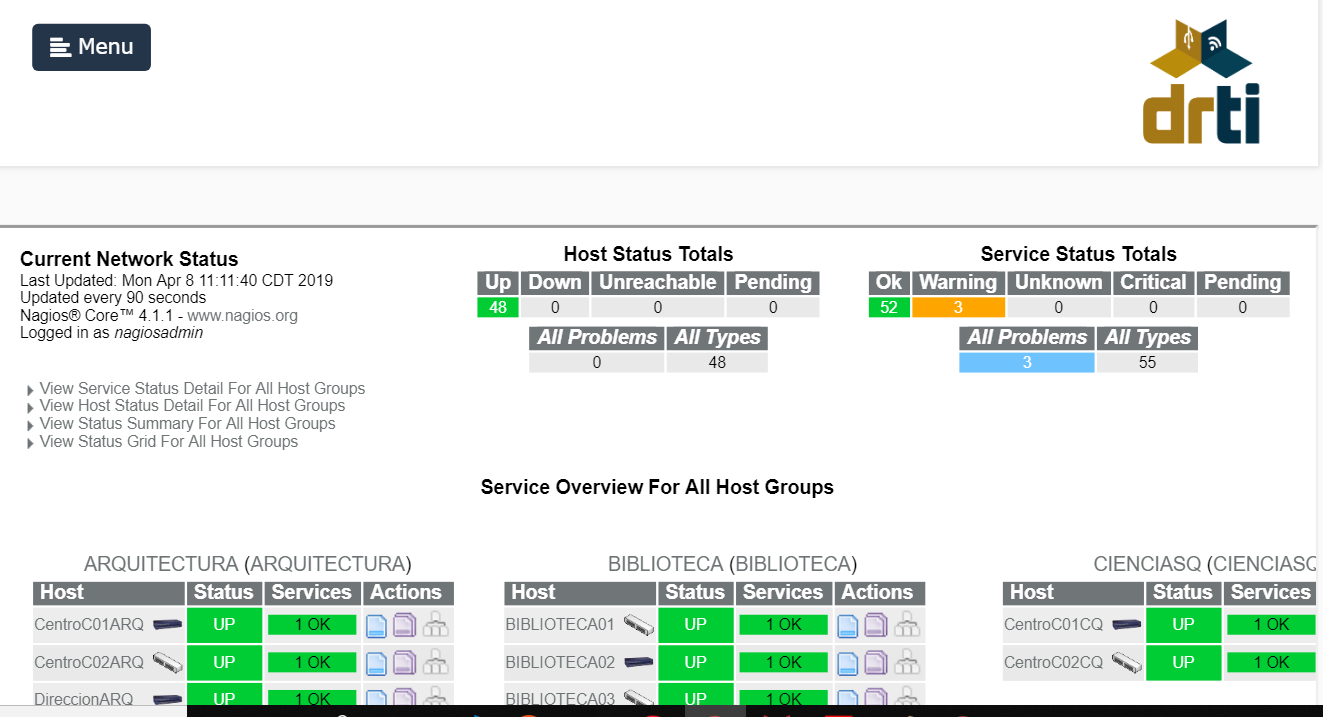
\includegraphics[width=0.8\textwidth]{./Imagenes/responsive.png}
      \caption{Nueva interfaz web de Nagios} \label{fig:Nagios-DRTI}
    \end{figure}
    \section{ Alertas por Correo Electrónico }
    Una de las características de Nagios es la de poder enviar notificaciones a ciertas personas cuando ocurre
    algo. Así, si un equipo esta apagado, tiene un problema de algún tipo, un servicio no funciona etc. Además
    de plasmarlo en la interfaz de Nagios, podrá enviar una notificación al personal oportuno.
    Como ya comentamos también es posible configurar un manejador de eventos, para que se ejecute algo
    cuando sucede cierta cosa. Sin embargo aquí nos centraremos únicamente en las notificaciones.
    Estas notificaciones o alertas pueden realizarse de muchos métodos, pero aquí solo veremos como
    configurarlas para el correo.
    \vspace{-5mm}
    \begin{alltt}
      \input{./txt/correo.txt}
    \end{alltt}
    \vspace{-10mm}
    Ya tenemos configurado Nagios y el correo, ya solo quedan los contactos. Si recordáis, en templates.cfg
    también había una plantilla para los contactos. Ahora vamos a ver qué son y como usarlos para recibir las
    alertas vía email.
    \vspace{-5mm}
    \begin{alltt}
      \input{./txt/correogroup.txt}
    \end{alltt}
    \vspace{-5mm}
    \begin{enumerate}
      \item {\bf service\_notification\_period: } Periodo de tiempo en el cual el contacto puede ser notificado
      \item {\bf host\_notification\_period: } Igual que el anterior pero para las notificaciones de los hosts.
      \item {\bf service\_notification\_options: } Tipo de notificaciones que serán enviadas para los servicios.
      \item {\bf host\_notification\_options: } Igual que el anterior pero con los estados de los hosts.
      \item {\bf service\_notification\_commands: } Comando que se ejecuta al enviar una notificación sobre un
      servicio.
      \item {\bf host\_notification\_commands: } Igual que el anterior pero para las notificaciones de los hosts.
    \end{enumerate}
    Los contactos al igual que otros objetos también tienen su fichero particular. En este caso es “ contacts.cfg” y
    en su interior ya viene definido un contacto llamado nagiosadmin. Nosotros nos quedaremos con este
    contacto tal como esta y únicamente editaremos el email.
    \vspace{-5mm}
    \begin{alltt}
      \input{./txt/contacto.txt}
    \end{alltt}
    \vspace{-5mm}
    Las directivas con las que viene definido ya nos deben sonar de otros objetos. Sin embargo existen algunas
    directivas más que no hemos visto aquí. Para obtener más información sobre estas y la definición de los
    contactos podéis leer la documentación.

      
\end{document}

